\documentclass[conf]{new-aiaa}
\usepackage{graphicx}
\usepackage{parskip}
\usepackage{amsmath}
\usepackage{float}
\usepackage{listings}
\usepackage{color}

\definecolor{mygreen}{rgb}{0,0.6,0}
\definecolor{mygray}{rgb}{0.5,0.5,0.5}
\definecolor{mymauve}{rgb}{0.58,0,0.82}

\lstset{ %
  backgroundcolor=\color{white},   % choose the background color
  basicstyle=\footnotesize,        % size of fonts used for the code
  breaklines=true,                 % automatic line breaking only at whitespace
  captionpos=b,                    % sets the caption-position to bottom
  commentstyle=\color{mygreen},    % comment style
  escapeinside={\%*}{*)},          % if you want to add LaTeX within your code
  keywordstyle=\color{blue},       % keyword style
  stringstyle=\color{mymauve},     % string literal style
}

\begin{document}

\title{Introduction to Optimization with OpenMDAO}
\author{Justin Gray}

\maketitle

\section{History of Optimization}


\noindent Though formal optimization theory is quite old, what we think of today as "optimization" is a fairly young discipline that emerged with the development of general purpose computing. 

    \begin{itemize}[itemsep=1.2em, label={}, itemindent=-3em]
        \item 1857: J. W. Gibbs shows that chemical equilibrium is attained when the energy is a minimum
        \item 1939: William Karush derives the necessary conditions for the inequality constrained problem in his Masters thesis. Harold Kuhn and Albert Tucker rediscover these conditions an publish their seminal  
            paper in 1951. These became known as the Karush–Kuhn–Tucker (KKT) conditions.
        \item 1959: Davidon develops the first quasi-Newton method for solving nonlinear optimization problems. Fletcher and Powell publish further developments in 1963.
        \item 1963: Wilson invents the sequential quadratic programming method for the first time. Han reinvents it in 1975 and Powell does the same in 1977.
        \item 1975: John Holland proposed the first genetic algorithm.
        \item 1977: Raphael Haftka publishes one of the first multidisciplinary design optimization (MDO) ap- plications, 
                in a paper entitled “Optimization of flexible wing structures subject to strength and induced drag constraints”[CITE].
        \item 1984: Narendra Karmarkar starts the age of interior point methods by proposing a more efficient algorithm for solving linear problems. In a particular application in communications network optimization, the solution time was reduced from weeks to days, enabling faster business and policy decisions. Karmarkar’s algorithm stimulated the development of several other interior point methods, some of which are used in current codes for solving linear programs.
        \item 1985: The first conference in MDO, the Multidisciplinary Analysis and Optimization (MA\&O) conference, takes place.
        \item 1995: Kennedy and Eberhart propose the particle swarm optimization algorithm
    \end{itemize}

    \subsection*{Why do we need optimization and what does ``gradient based'' mean?}
        
        Optimization is a technique for finding solutions --- the design variables --- that maximize or minimize some quantity of interest  --- the objective function. 
        Fundamentally, the need for optimization arises when you are dealing with under-defined problems; when you have more degrees of freedom than equations to constrain them with. 

        Examples: 
        \begin{itemize}
            \item Find the minimum value of a parabola
            \item What are the angle of attack and chord length needed to get a 5 Newtons of lift for a NACA 0012 airfoil
        \end{itemize}

        The objective function provides a means of distinguishing one solution from another, 
        and thus by seeking the max or min of the objective you have fundamentally converted an under-defined problem into a well defined one. 

        All optimizers perform this task, though they do so in a variety of different ways. 
        There are three main classes of optimization algorithms: 
        
        \subsubsection{Brute Force}
            If your objective function is cheap enough and the number of design variables is small enough, then you can simply enumerate the entire design space and pick the best design out of the set of solutions you found. 
            If your design variable are continuous, you can just pick a very fine discretization to sample with. 

            There are some very nice aspects of this approach. For one thing, you get a whole lot more information than just what the best design is, since you know the answer for all the designs. 
            For another, this approach is dead simple and highly parallel. 
            Perhaps most importantly, within your defined design space, this is the only method that can gurantee that you will find the overall best answer, or the global optimum. 

            If you can afford to use a brute-force technique, you should! As a rule of thumb, if you have 3 or less variables and a function that runs in under 0.01 seconds, then consider this approach. 

        \subsubsection{Gradient-free}
            As the name suggests, these methods do not require any gradient information to perform optimization.
            Some methods, such as the simplex algorithm and the Constrained Optimization by Linear Approximation (COBYLA), are mathematically rigorous approaches to solving optimization problems. 
            Other methods, such as the massive set of evolutionary algorithms (e.g. genetic algorithms and partical swarm algorithms), are heuristic in nature and do not necessarily rest on a rigorous mathematical footing. 

            Regardless of the mathematical underpinnings of these methods, they can be quite useful. 
            Like the brute force method they are typically very easy to implement and very highly parallel, but they can typically work on problems with as many as 10-20 design variables even if the cost of that computing the objective function is much higher. 
            There are some advanced gradient-free methods that can even scaled up to 100 variables with reasonable performance. 
            Another important characteristic of gradient-free methods is that they are suitable for use even when some design variables are discrete. 

            Despite the many good qualities of gradient-free methods, they tend to require a large number of function evaluations to get a reasonable answer. 
            They also commonly include some stochastic qualities that make it so you will get a different answer each time you run them. 
            This is why you will often see results from gradient free methods presented as an average (or some other statistical quantity) taken over multiple runs. 

            Here are some good gradient-free methods that you can look into: 
            \begin{itemize}
                \item COBYLA: Constrained Optimization by Linear Approximation
                \item EGO: Efficient Global Optimization 
                \item NSGA-II: Non-dominated Sorting Genetic Algorithm II
                \item ALPSO: Augmented Lagrangian Particle Swarm Optimization
            \end{itemize}Improvement of efficient global optimization with application to aircraft wing design

        \subsubsection{Gradient-based}

            Gradient-based optimization methods use derivative information to formally transform an under-defined problem into a well-defined one.  
            Recent research has shown that for problems with over 100 design variables, gradient based methods are 2-4 orders of magnitude faster than gradient-free methods. 
            The improved computational performance is the primary motivation for using gradient-based optimization algorithms. 
            
            Of course, there is no free lunch! The downside to using gradient-based optimization algorithm is that it can be quite difficult to compute the gradients that you need. 
            All of the promised performance of gradient-based methods falls apart if you can not compute accurate derivative information in a computationally efficient manner. 
            It is also important to note that, since the definition of a derivative fundamentally assumes a continuous function and a continuous design space, these methods can only work on continuous problems. 

            Another potential limitation of gradient-based methods is that they can only find ``local optima'', and hence are less effective at searching bumpy design spaces. 
            In other words, gradient-based methods are very efficient at climbing whatever hill the initial guess has started them on but they will not search any other hills even if they might have taller peaks. 

            Despite the challenges associated with computing derivatives, the limitation to continuous design spaces, and the local nature of the algorithms, when properly implemented the performance of gradient-based methods is so great that it justifies their use even for relatively small optimization problems. 
            Gradient-based methods are the only class of optimization algorithms that can handle 1000's, 10,000's, or even 1,000,000's of design variables. 

\section{What is OpenMDAO and why would you use it?}

    MDAO stands for ``Multidisciplinary Design Analysis and Optimization'', though you may see ``Multidisciplinary Design Optimization'' (MDO) used interchangeably. 
    In 2008 the OpenMDAO project was originally conceived to develop an open-source computational framework to support the broad application of state-of-the-art gradient-free and gradient-based MDAO methods. 

    Today, OpenMDAO is a general purpose computing library that handles data-passing, parallel communication, and provides a library of efficient useful tools for general engineering model building and optimization. 
    The framework can integrate analyses across the fidelity spectrum and can work with both serial and distributed memory analysis tools such as CFD and FEA. 
    These capabilities make the framework a good platform for building complex models and generic modeling libraries on top of, and they provide all the needed functionality to make use of gradient-free optimization. 

    The most unique feature of OpenMDAO is its ability to automatically and efficiently compute derivatives across complex multi-disciplinary models. 
    No other tool offers the same level of flexibility and automation of implementation that OpenMDAO does. 
    This makes it possible for non-experts to employ the most efficient derivative computation techniques available today, thus dramatically lowering the activation energy required to make the best use of gradient-based optimization methods. 

    So, while OpenMDAO has many useful features employing for gradient-free methods, what sets it apart is its support for gradient-based methods. 
    By employing gradient-based optimization with OpenMDAO you can take advantage of the 2-4 order of magnitude speed ups that are promised by researchers in the field, without actually having to become an expert. 

    In this lesson, we'll introduce some of the underlying theory for computing derivatives and you will see why it can be so challenging and labor intensive to do manually. 


\section{Introduction to the Theory Behind Gradient-Based Optimization}

    \subsection{Unconstrained Optimization}
    Consider a simple parabolic function of one variable: 
    \begin{equation}
        f = F(x_1) = (x_1 - 3)^2 + x_1 - 3 \ . 
    \end{equation}
    If I asked you to ``find the value of $f$'', then you have an under-defined problem. 
    There is an infinite number of solutions for $f$, corresponding to the infinite number of values that $x_1$ can take. 
    If instead, I ask you to ``find the minimum of value $f$'', you now have a well-defined problem.    
    The formal optimization problem statement for this would be: 

    \begin{table}[H]
        \centering
        \begin{tabular}{lc}
            \hline
            min. & $f$ \\
            w.r.t & $x$ \\ \hline
        \end{tabular}
    \end{table}


    Since this function is parabolic, we know that there is one and only one minimum for all values of $x_1$. 
    From basic calculus, we know that we can find the minimum of $f$ by taking the derivative and setting the resulting expression equal to 0. 
    \begin{equation}
        \frac{\partial f}{\partial x_1} = 2(x_1 - 3) + 1 = 0 \ . 
    \end{equation}

    Now lets look at a parabolic function of two variables: 
    \begin{equation}
        f = F(x_1,x_2) = (x_1 - 3)^2 + x_1 x_2 + (x_2 + 4.0)^2 - 3 \ . 
    \end{equation}

    Since it is still parabolic we know that there is still only one minimum. 
    $f$ is still a scalar, but now the input is 2 scalars: $x_1$ and $x_2$
    To find the minimum, we take the derivative of $f$ with respect to the two $x$ variables and set the result equal to 0. 
    Because there are two inputs, instead of a single equation we get a system of two equations. 
    \begin{align}
        \frac{\partial f}{\partial x_1} &= 2(x_1 - 3) + x_2 = 0 \notag \\
        \frac{\partial f}{\partial x_2} &= x_1 + 2(x_2 + 4.0) = 0 \label{eq:linear_deriv}
    \end{align}
    Now we can solve this system of equations for $x_1$ and $x_2$ to find the minimum of the original objective function. 
    This is referred to as an \textbf{implicit function}, which would generally be represented as: 
    \begin{equation} 
    r = \mathcal{R}(x_1, x_2) = 0 \ . 
    \end{equation}
    It is implicit because you do not explicitly compute the values $x_1$ and $x_2$, but rather we solve the residual equation and when that solution is found we also know the desired values. 


    Equation~\eqref{eq:linear_deriv} can be re-arranged into a linear system of equations: 
    \begin{equation}
        \begin{bmatrix}
        2,1 \\
        1,2
        \end{bmatrix} 
        \begin{bmatrix}
        x_1 \\ 
        x_2
        \end{bmatrix} = 
        \begin{bmatrix}
        6 \\ 
        -8
        \end{bmatrix} \ .
    \end{equation}
    We can now solve this linear system by inverting the matrix on the left hand side, to find the values of $x_1$ and $x_2$ that will minimize the original paraboloid objective function.
    So for this specific case, with a parabolic objective function, it turns out the there is also an explicit form for the nonlinear system of equations needed to find the minimum. 

    What if the objective function is cubic though? 
    \begin{equation}
        f = F(x_1,x_2) = (x_1 - 3)^2 + x_1^2 x_2 + (x_2 + 4.0)^2 - 3 \ . 
    \end{equation}
    We made it cubic my modifying the cross term ($x_1^2 x_2$), and so now the system of equations to find the minimum will be: 
    \begin{align}
        \frac{\partial f}{\partial x_1} &= 2(x_1 - 3) + 2 x_1 x_2 = 0 \notag \\
        \frac{\partial f}{\partial x_2} &= x_1^2 + 2(x_2 + 4.0) = 0 \ .
    \end{align}
    Since this system of equations is nonlinear, we can no longer represent it in a simple matrix form and solve it with a simple matrix inverse. 
    This had two important consequences. 
    First, since this system of equations is now second order we know that there will be two roots which means there are two minimum values. 
    Also, and perhaps more importantly, we now need to employ a a nonlinear solution technique to find those roots. 
    For a simple problem like this, perhaps you can find the roots by hand using substitution. 

    What if your objective is a cubic function 1000 variables? 
    \begin{equation}
        f = F(x_1,x_2, ..., x_{1000}) = F(\bar{x}) \ . 
    \end{equation}
    Now, to find the minima we will have to solve a nonlinear system of 1000 equations: 
    \begin{equation} 
    r = \mathcal{R}(x_1, x_2, ...,  x_{1000}) =  \mathcal{R}(\bar{x}) = \frac{\partial f}{\partial \bar{x}} =  0 \ . 
    \end{equation}
    This is far to large to solve by hand, but the implicit form of the equations can be solved using a numerical technique such as Newton's method. 
    Newton's method is composed of the iterative solution to the following equation: 
    \begin{equation}
         \Delta \bar{x} = - \left[\frac{\partial \mathcal{R}}{\partial \bar{x}} \right]^{-1} \bar{r} \ , 
    \end{equation}
    where $\left[\frac{\partial \mathcal{R}}{\partial x} \right]$ is a matrix of partial derivatives computed about some $\bar{x}^*$, $\left[\Delta x\right]$, $\bar{r}$ is the vector residual values computed at $\bar{x}^*$, and $\Delta \bar{x}$ is the update that should be applied to $\bar{x}^*$ for the next iteration. 

    Note that we now need $\frac{\partial \mathcal{R}}{\partial \bar{x}}$, but $\mathcal{R}$ was itself defined as a partial derivative of $f$ with respect to $\bar{x}$. 
    So now that means that we now need second-derivatives with respect to $f$: 
    \begin{equation}
         \left[\frac{\partial \mathcal{R}}{\partial \bar{x}} \right] =  \left[\frac{\partial^2 f}{\partial \bar{x}^2} \right] \ . 
    \end{equation}
    $\frac{\partial^2 f}{\partial \bar{x}^2}$ is called the Hessian matrix of $f$.
    This is how, for an unconstrained optimization, we can create a well-defined problem (same number of unknowns as equations to constrain them) by taking derivatives of the objective function with respect to the design variables. 

    If the system of equations we get by taking those derivatives is nonlinear, then we need to Newton's method to iteratively solve for roots that will minimize the objective.  
    If $\bar{x}$ is a length 1000 vector, The Hessian of $f$ will be $1000 \times 1000$, 
    so there are one million terms in the Hessian. 
    We would need to derive a formula for each of those terms in order to implement Newton's method and solve the optimization problem. 

    Obviously, deriving one million equations isn't feasible. 
    For smaller problems, you could maybe compute the Hessian by hand --- in fact, this is what J.W. Gibbs did to solve for chemical equilibrium in 1857.
    However, for general problems, there is a suite of non-linear optimization methods (e.g. sequential quadratic programming and interior point methods) have been developed so that we either don't need the Hessian at all or don't have to explicitly compute it. 
    Some optimization algorithms, called quasi-Newton methods, approximate the Hessian using only first derivative information.

    So, while you most likely do not need to explicitly compute the Hessian, you still need to compute the first-derivatives of the objective function with respect to the design variables. 
    So for 1000 variable unconstrained optimization we would still need to derive 1000 formulas. 
    This is certainly much more achievable, but clearly still a lot of work. 

    \subsection{Constrained Optimizations}
        
    Practically speaking, optimization problems are very rarely unconstrained. 
    Usually, you want to maximize or minimize an objective function, subject to some set of constraints. 
    While an unconstrained optimization problem is under-defined (more unknowns than equations to define them), 
    a constrained optimization problem can actually be under-defined, well-defined, or even over-defined (less variables than equations to define them). 
    It all depends on how many constraints you have in your problem, compared to how many design variables. 
    You can have equality constraints ($g(x) = 0$), or inequality constraints ($h(x) < 0$). 
    Both are broadly handled the same way, though there are some slight differences. 


        \subsubsection{Equality constraints: $h = H(x) = 0$}
        First we will modify the optimization problem statement to include the constraints. 
        \begin{table}[H]
            \centering
            \begin{tabular}{lc}
                \hline
                min. & $f$ \\
                w.r.t & $x$ \\ 
                subject to & $h = 0$ \\ \hline 
            \end{tabular}
        \end{table}

        Our previous technique for minimizing a function will not work here, because the derivatives of the objective function do not take the constraints into account at all. 
        But we can modify the problem a bit in order to take both the objective and the constraints into account by forming what is called the Lagrangian:  
        \begin{equation}
            \mathcal{L}(x) = F(x) - \lambda H(x) \ .
        \end{equation}
        The Lagrangian condenses the constrained optimization problem, which was composed of multiple separate equations, back into a single scalar equation which we can apply our existing derivative based technique to! 
        In order to do this, we've introduced a new set of unknown variables, $\lambda$, to the problem --- one for each equality constraint we want to consider. 
        The set of $\lambda$ variables are called the Lagrange multipliers, and they provide the necessary additional degrees of freedom to keep the problem well-posed (we'll see why they are needed in a bit). 
        You can take derivatives of the Lagrangian function, with respect to all of the unknown variables ($x$ and $\lambda$), and set them equal to 0 for form a system of equations that can be solved to find minima. 


        The Lagrange multipliers are additional unknown variables who's values must be solved for, but from an engineering perspective they are not new design variables in the problem. 
        So you might be tempted to think they are merely mathematical tricks to maintain the well-posedness of the problem. 
        However, they do have some physical meaning. 
        The Lagrange multipliers represent the sensitivity of the optimum objective value to the constraint. 
        So a very large Lagrange multiplier indicates that the solution is very sensitive to the constraint, and vice versa. 


        Lets differentiate the Lagrangian with respect to all the unknown variables ($\lambda$ and $x$) and set the equations equal to 0: 
        \begin{alignat}{3}
            \frac{d\mathcal{L}}{d\lambda} &= \frac{dH}{dx} &&= 0 \label{eq:dLdlambda} \\
            \frac{d\mathcal{L}}{dx} &= \frac{dF}{dx} - \lambda \frac{dH}{dx} &&= 0 \label{eq:dLdx}
        \end{alignat}
        Because of Equation~\eqref{eq:dLdlambda}, solutions to this system of equations with clearly have to satisfy the equality constraints. 
        Equation~\eqref{eq:dLdx} is what actually minimizes the Lagrangian.
        If we have $N_h$ constraints, then  Equation~\eqref{eq:dLdlambda} is actually a set of $N_h$ equations. 
        If we have $N_x$ design variables, then Equation~\eqref{eq:dLdx} is a set of $N_x$ equations. 
        In total, this gives us $N_h + N_x$ equations, for which we need an equal number of degrees of freedom. 
        This is why the Lagrange multipliers are necessary to be able to solve constrained optimization problems. 
        Without them, the system of equations you get from differentiating the Lagrangian would be over-defined. 

        To solve 


        \subsubsection{Inequality constraints: $g = G(x) \ge 0$}

        Again, lets modify the optimization problem to include the inequality constraint. 
        \begin{table}[H]
            \centering
            \begin{tabular}{lc}
                \hline
                min. & $f$ \\
                w.r.t & $x$ \\ 
                subject to & $g \ge 0$ \\ \hline 
            \end{tabular}
        \end{table}

        Inequality constraints are tricky because they may or may not actually constrain the final solution. 
        If your final answer is constrained, inequality constraints actually behave just like an equality constraints. 
        However, if the overall optimum exited at a point where, for example, g=1000 then the inequality constraint actually had no impact on the solution at all! 

        We can introduce a vector of slack variables, $\xi$, to the inequality constraints to convert them into equality constraints: 
        \begin{table}[H]
            \centering
            \begin{tabular}{lc}
                \hline
                min. & $f$ \\
                w.r.t & $x, \xi$ \\ 
                subject to & $g + \xi = 0$ \\ 
                           & $\xi < 0$ \\ \hline
            \end{tabular}
        \end{table}
        For this modification to be valid, we need to ensure that $\xi$ always takes on whatever value is necessary to enforce the constraint if it is active, but if the constraint is inactive then $\xi$ should have no impact on the solution. 
        It is not obvious that things will work out this way from the given formulation, but luckily they do once we form the Lagrangian. 
        \begin{align}
            \mathcal{L}(x,\xi) &= F(x) + \lambda(G(x) + \xi) \notag \\
                               &= F(x) + \lambda(G(x)) + \lambda \xi \label{eq:L_ineq}
        \end{align}

        Similar to before, we can take derivatives of the Lagrangian with respect to $x$ and $lambda$, which will yield 
        $N_x+N_g$ equations. 
        However, now we run into a problem because we have introduced an additional set of $N_g$ slack variables to the problem and so we still have an under-defined set of equations. 
        In other words, we don't have any equations to constrain the values for the slack variables, so we can not yet solve for solutions that minimize the Lagrangian. 

        You might be tempted to simply differentiate with respect to $\xi$, since thats what we have done in all the previous cases. 
        But, a quick look shows that this will not work.
        \begin{equation}
            \frac{d\mathcal{L}}{d\xi} = \lambda \label{eq:dL_dxi}
        \end{equation}
        The only way for Equation~\eqref{eq:dL_dxi} to equal zero is if $\lambda=0$, which is not at all what we want. 
        Rather than adding an additional equation to constraint $\xi$, instead our additional equation has actually removed the necessary additional degree of freedom that $\lambda$ introduced in the first place. 
        So, to avoid this situation we need to find another way to constrain $\xi$. 

        Take another look at the $\lambda \xi$ term in Equation~\eqref{eq:L_ineq}. 
        Since $\xi$ is a free variable which must be less than 0 then we could set $\xi=-\infty$ and then $\mathcal{L}=-\infty$
        . 
        This is obviously a degenerate solution that we want to avoid, so to exclude it we can see that if $\xi \ne 0$ then $\lambda = 0$. 
        Similarly, $\lambda$ is also a free variable so that if it $\lambda\ne0$, then $\xi=0$. 
        So, in order to avoid these degenerate solution with $\mathcal{L}=-\infty$, we must enforce what is called the complementary slackness condition: 
        \begin{equation}
            \lambda \xi = 0 \ , 
        \end{equation}
        that ensures that one or the other of the two variables must be 0. 
        The complimentary slackness condition gives us an additional $N_g$ equations, which means we now have a well-defined problem formulation that can be solved to find minima: 
        \begin{align}
            \frac{dG}{dx} &= 0 \\
            \frac{dF}{dx} - \lambda \frac{dG}{dx} &= 0 \\
            \lambda \xi &= 0
        \end{align}


    \subsection{Summary}
    Gradient-based optimization transforms an under-defined problem into a well-defined implicit function that can be solved using nonlinear solution methods by taking derivatives of the Lagrangian function and setting the resulting equations equal to 0. 
    This forms a system of equations that can be solved using nonlinear solution techniques, such as Newton's method. 

    In reality, not many numerical optimization algorithms actually directly solve this nonlinear system because it requires too much work to compute the Hessian. 
    None the less, even if an optimizer does not directly solve this system of nonlinear equations it is still searching for solutions to it. 
    Hence, we have gone over this material so that you can understand how an optimizer sees the problem you are posing to it. 

    \section{Taking Derivatives of Outputs of Implicit Functions}

    We have seen how gradient-based optimization can create a system of implicit equations by taking derivatives of the objective function and constraints and we've also discussed briefly how Newton's method could be used to solve that system of equations, if you were willing to compute the actual Hessian matrix.
    If you do not wish to form the exact Hessian, then many gradient based optimization algorithms exist that don't require it, 
    but they all will still require derivatives of the objective function and constraints with respect to the design variables. 

    Up to this point all the examples that we've considered provided the objective and constraint functions as explicit functions. 
    In other words, we say that the objective, $f$, can be computed directly by evaluating the function $F(x)$. 
    Inherent in that description of the function is the idea that there is an exact, analytic solution for $F$ given any value of $x$. 
    While this situation is certainly true for simple polynomial expressions, and also for some kinds of more complex engineering analyses, 
    the reality is that the vast majority of modern engineering computations include implicit calculations. 
    For example CFD and FEA analyses are implicit and turbine engine cycle analysis is highly implicit. 
    Tools such as COMSOL, a popular multiphysics solver, is also implicit in nature. 

    A general implicit function can be represented as 
    \begin{equation}
        R(x,y) = 0 \ , 
    \end{equation}
    where $R$ is the residual function, $x$ is the set of fixed inputs, and $y$ is the set of implicit output variables that must be solved for given any specific values for $x$. 
    There can be any arbitrary number of input variables, but there must always be the same number of residuals as there are implicit variables. 

    We refer to $y$ as the implicit outputs, because they are the values that actually get solved for when the residuals are all equal to 0.
    In some cases, your objective function or constraint might be one of those $y$ values. 
    For example, what if you wanted to minimize the mass of a clamped beam with a load applied at the end, by varying the material thickness along the beam, subject to a limit on the displacement of the beam at the tip. 
    \begin{table}[H]
        \centering
        \begin{tabular}{lcc}
            \hline
            min. & $m$ & mass (kg)\\
            w.r.t & $t$ & material thickness (mm) \\ 
            subject to & $u < 4$ & displacement (cm)\\ \hline
        \end{tabular}
    \end{table}
    The mass of the beam $m$ can be directly computed as a function of the thickness design variables. 
    But the displacement of the beam ($u$), which will be used as a constraint, is the implicit output of a FEA analysis. 
    So we have no explicit form for out constraint value, but we still need to compute derivatives of it with respect the design variables. 
    In other words, we need to compute $\frac{du}{dt}$, when the only definition we have for $u$ is $R(t,u)=0$.

    \subsection{Explicit vs Implicit Functions}
    Before we dive into ways to compute the derivative of implicit functions, it is worth spending some time examining the difference between implicit and explicit and functions more closely. 
    Both types of functions have inputs and outputs, but the manner in which they compute the outputs is vastly different. 
    Moreover, any explicit function can be written in an equivalent implicit form but not all implicit functions have an equivalent explicit form. 

    Consider the example of the Mach-Area relationship for compressible, isentropic flow: 
    \begin{equation}
        \frac{A}{A^*} = \left(\frac{\gamma+1}{2}\right)^{-\frac{\gamma+1}{2(\gamma-1)}} 
                        \frac{1}{MN} 
                        \left( 1 + \frac{\gamma-1}{2}MN^2 \right)^{\frac{\gamma+1}{2(\gamma-1)}} \ ,
                        \label{eq:mach_area}
    \end{equation}
    where N$A$ is the flow area, $A^*$ critical flow area at Mach=1, $MN$ is the Mach number of the flow, and $\gamma$ is the ratio of specific heats that we'll assume to be a constant ($\gamma=1.4$ is a very good assumption except at really high temperatures).

    Equation~\eqref{eq:mach_area} is an explicit function that computes the area ratio $A/A^*$ directly, given any value for $MN$. 
    You can easily plot the relationship between the two --- check out the example code given in Figure~\ref{fig:mach-area}. 
    However, if we flip the question around and ask "For a given area ratio, what is the Mach number?" we will find that there is no longer an explicit relationship because there is no way to isolate $MN$ by itself. 
    \begin{figure}[H]
        \centering
        \lstinputlisting[language=Python]{mach_area.py}
        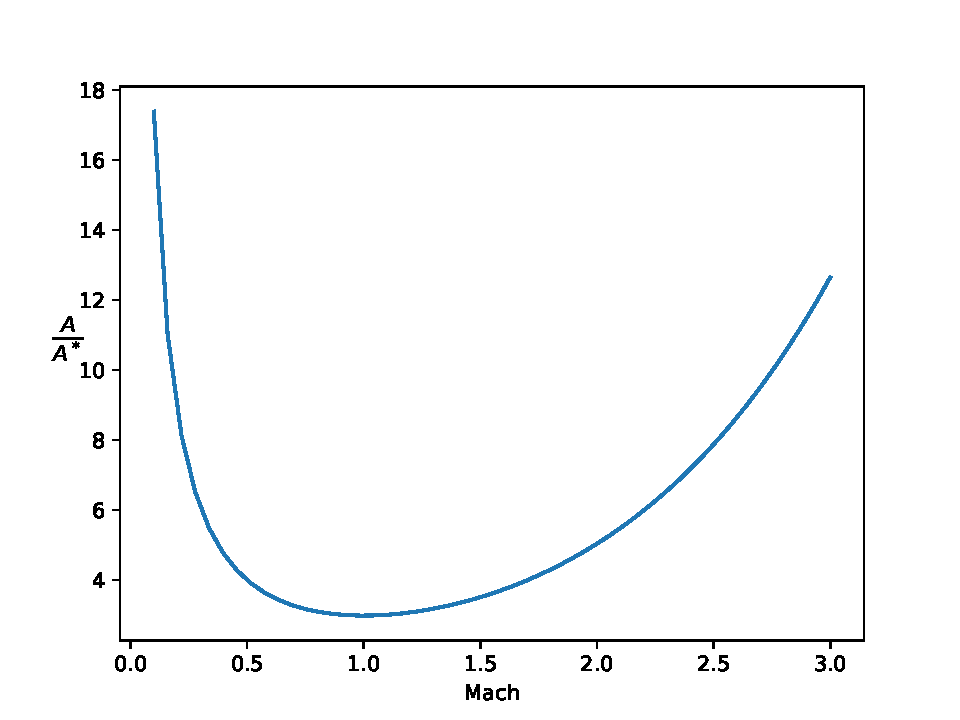
\includegraphics[width=.75\textwidth]{mach_area.pdf}
        \caption{Python code plotting the Mach-area relationship}
        \label{fig:mach-area}
    \end{figure}

    So, if you wanted to solve for the Mach number that matches a given area ratio you need to use a Nonlinear solver. 
    In order to do that, you need to define a residual function that must be driven to 0: 
    \begin{equation}
        R(\frac{A}{A^*}, MN) = \frac{A}{A^*} - \left[ \left(\frac{\gamma+1}{2}\right)^{-\frac{\gamma+1}{2(\gamma-1)}} 
                        \frac{1}{MN} 
                        \left( 1 + \frac{\gamma-1}{2}MN^2 \right)^{\frac{\gamma+1}{2(\gamma-1)}}\right] = 0
                        \label{eq:implicit_mach_area}
    \end{equation}
    Equation~\eqref{eq:implicit_mach_area} is litarally just a re-arranging of Equation~\eqref{eq:mach_area} by moving the right hand side over to the left. 
    So they are exactly the same, but the implicit form is more useful since it can be solved for either area ratio or Mach number, while the explicit form can only be solved for area ratio. 
    Figure~\ref{fig:mach-area-implicit} give you a short bit of python code that can apply Newton's method to solve the implicit form of this equation. 
    Notice that the answer you get from Newton's method is dependent on the initial guess you give to the
    \begin{figure}[H]
        \centering
        \lstinputlisting[language=Python]{mach_area_solve.py}
        \caption{Python code solving the implicit Mach-area equation using newton's method}
        \label{fig:mach-area-implicit}
    \end{figure}

    The trick of re-arranging terms to form an implicit version from explicit function works for any general function.
    Hence we can generally say that all explicit functions have an implicit form, but not all implicit functions have an explicit form. 
    We're discussing this subtlety because internally and out of sight from the users, OpenMDAO represents all functions in their implicit form. 
    As a user you don't need to worry about this transformation --- it is managed automatically for you --- but the fact that it occurs becomes relevant when trying to understand how OpenMDAO computes derivatives across complex models.  
    So we'll revisit this subject a bit later. 


    \subsubsection{Disguising an implicit function as an explicit one}
    Of more direct relevance to you as a user is that you can disguise an implicit function in an explicit form. 
    To be perfectly clear, this is \textbf{not} the same thing as converting an implicit function into an equivalent explicit form! 

    The word ``disguise'' is used very intentionally here. What you can do is put a black-box wrapper around an implicit function to make it look like an explicit one, even though the internal calculation is still being performed in an implicit way. 

    Lets go back to our example to see this in action, solving for Mach number when given an area ratio. 
    The implicit form is given in by Equation~\ref{eq:implicit_mach_area}. 
    We're \textbf{not} going to change that at all. 
    However, if look at the code in Figure~\ref{eq:implicit_mach_area} you see that we can get solutions with a single call to the `newton' method. 
    Now, with a few more lines of code, we can wrap that whole process up into something that looks like a regular explicit function, as shown in Figure~\ref{fig:mach-area-fake-explicit}. 
    \begin{figure}[H]
        \centering
        \lstinputlisting[language=Python]{mach_area_fake_explicit.py}
        \caption{Disguising an implicit function with an explicit wrapper}
        \label{fig:mach-area-fake-explicit}
    \end{figure}

    Even though the functions look explicit now, they aren't really. 
    Why does this matter? 
    For one thing, if the function was really explicit then you would expect to be able to give it any allowable value for area ratio --- anything over 1.0 --- and expect to get an answer back. 
    However, if you experiment a bit with that function you'll see that the nonlinear solver isn't that stable. 
    It gets an answer for $A/A^*=3.0$, but not for $A/A^*=2.5$. 
    A second reason, which is especially important in the context of optimization, is that the way in which you need to compute derivatives across the function changes because of the implicitness. 
    We'll talk about this in more detail in the next sections. 




    % \subsection{Using Newton's method to solve implicit functions}

    % Given a general implicit function, $r=R(x,y)$, we want to solve for the implicit output variables $y$ such that $r=0$. 
    % A single iteration of Newton's method is given as: 
    % \begin{equation}
    %    \left[\frac{\partial \mathcal{R}}{\partial y} \right] \Delta y = -r \ ,
    % \end{equation}
    % and then we just iteratively apply this step till we reach sufficient convergence. 

    % For the implicit Mach-area relationship: 
    % \begin{equation}
    %     R(\frac{A}{A^*}, MN) = \frac{A}{A^*} - \left[ \left(\frac{\gamma+1}{2}\right)^{-\frac{\gamma+1}{2(\gamma-1)}} 
    %                     \frac{1}{MN} 
    %                     \left( 1 + \frac{\gamma-1}{2}MN^2 \right)^{\frac{\gamma+1}{2(\gamma-1)}}\right] = 0
    %                     \label{eq:implicit_mach_area}
    % \end{equation}
    % we can compute the necessary derivative analytically: 
    % \begin{equation}
    %     \frac{\partial R}{\partial MN} = \left(\frac{\gamma+1}{2}\right)^{-\frac{\gamma+1}{2(\gamma-1)}} 
    %     \left[\frac{1}{MN^2} \left( 1 + \frac{\gamma-1}{2}MN^2 \right)^{\frac{\gamma+1}{2(\gamma-1)}} - 
    %        \frac{\gamma+1}{2(\gamma-1)}\left( 1 + \frac{\gamma-1}{2}MN^2 \right)^{\frac{\gamma+1}{2(\gamma-1)} - 1}(\gamma-1)
    %     \right] 
    % \end{equation}

    \subsection{Numerical approximation of derivatives}
    Numerical approximation of derivatives is by far the most common approach used by engineers in practice. 
    Most optimizers and solvers that require derivative information come with built in numerical approximation methods to use by default. 
    The primary advantage of these numerical approximations is that they are very easy to implement.
    The primary disadvantage is that they are expensive and can be very accurate. 

    The first order forward difference approximation is given by: 
    \begin{equation}
        \frac{dF}{dx} \approx \frac{F(x+\epsilon) - F(x)}{\epsilon}
    \end{equation}
    This can be derived by looking at a Taylor expansion of $F(x)$
    \begin{align}
        F(x+\epsilon) &= F(x) + \frac{dF}{dx}\epsilon + \frac{1}{2}\frac{d^2F}{dx^2}\epsilon^2 + ... \\
        \frac{dF}{dx}\epsilon &= F(x+\epsilon) - F(x) - \frac{1}{2}\frac{d^2F}{dx^2}\epsilon^2 - ... \\
        \frac{dF}{dx} &= \frac{F(x+\epsilon) - F(x)}{\epsilon} - \frac{1}{2}\frac{d^2F}{dx^2}\epsilon \\
        \frac{dF}{dx} &\approx \frac{F(x+\epsilon) - F(x)}{\epsilon}
    \end{align}
    In the last step, we neglect any terms multiplied by $\epsilon$ because it is small so we can assume that these terms are insignificant. 
    Thus we get an approximation for the derivative with error that varies with directly $\epsilon$. 
    This is why its called a first-order approximation. 

    You have to compute this approximation once for every variable that you want to take a derivative with respect to. 
    So the compute cost scales linearly with the number of input variables you're considering. 

    What about accuracy?
    In theory, you can just take $\epsilon$ to be really tiny and we can get a very accurate derivative approximation. 
    In practice though, we run into a problem when $\epsilon$ gets too small.
    Lets look a a simple explicit example function: $sin(x)$ at $x=\pi/4$.
    If we look at a sweep of step sizes from $10^{-2}$ to $10^{-15}$, and compare the FD approximation to the analytic answer ($cos(x)$), 
    then the relative error follows the trend shown in Figure~\ref{fig:fd_subtractive_cancellation}.
    \begin{figure}[H]
        \centering
        \lstinputlisting[language=Python]{sin_fd.py}
        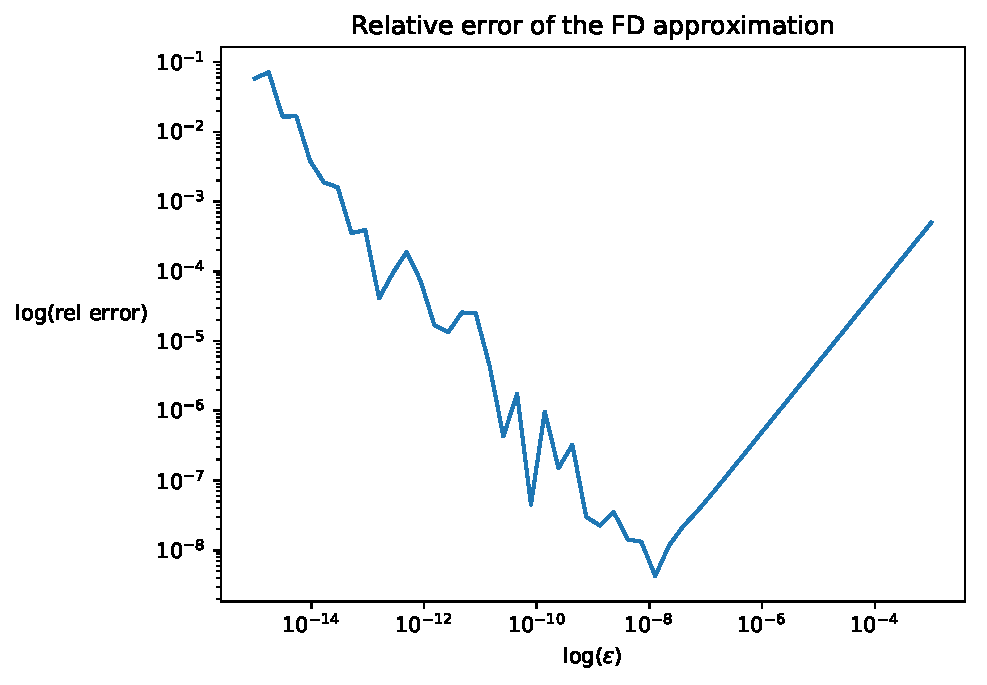
\includegraphics[width=.75\textwidth]{sin_fd.pdf}
        \caption{Relative error of the first order FD approximation for $\frac{d sin(x)}{dx}$ vs step size ($\epsilon$)}
        \label{fig:fd_subtractive_cancellation}
    \end{figure}
    Between $10^{-4}$ and about $10^{-8}$ we get the linear trend we expect --- the error is going down in direct proportion to the decrease in $\epsilon$. 
    For step sizes smaller than $10^{-8}$ though, the error starts to climb and eventually gets quite large. 
    The theory says the error should continue to decrease as $\epsilon$ decreases, 
    but the code says that we're limited in precision after a certain point. 

    Why is there a difference between theory and numerical reality? 
    The discrepancy arises because computers use finite-precision math (i.e. floating point math), 
    and this phenomenon is called subtractive cancellation. 
    Essentially, because computers don't represent floating point numbers with infinite precision there is a limit to how small of difference they can resolve in two numbers. 

    Practically, what this means is that there is always going to be a lower-limit on how accurate your numerical derivative approximation can be. 
    The more non-linear the function the smaller the $\epsilon$ that you would need need in theory, but the subtractive cancellation phenomena is always going to limit how small you can go. 

    \subsubsection*{Can we do anything to get around subtractive cancellation?}

    Yes! You have two options. 

    1) Use a higher order FD approximation, like central-difference. 
    This will give second-order convergence, which means that the error in the derivative will be proportional to $\epsilon^2$. 
    In other words, for the same $\epsilon$ you get a much smaller error. 

    2) Don't use subtraction! Seriously...

    Lets look at a Taylor expansion for $F(x+\epsilon i)$ --- so we're looking at complex arithmetic now. 
    \begin{align}
        F(x+\epsilon) &= F(x) + \frac{dF}{dx}\epsilon i + \frac{1}{2}\frac{d^2F}{dx^2} (\epsilon i)^2 +  \frac{1}{6}\frac{d^3F}{dx^3} (\epsilon i)^3 + ... \\
        F(x+\epsilon) &= F(x) + \frac{dF}{dx}\epsilon i - \frac{1}{2}\frac{d^2F}{dx^2} \epsilon^2 +  \frac{1}{6}\frac{d^3F}{dx^3} \epsilon^3 i + ... \label{eq:complex_taylor}
    \end{align}
    Notice that in the right hand side of Equation~\eqref{eq:complex_taylor} some of the terms are real and some of the terms are complex. 
    In particular, the second order term that includes $d^2F/dx^2$ is real and negative because $i^2=-1$.  
    Similarly, the third order term is negative because $i^3=-i$.
    We can split Equation~\eqref{eq:complex_taylor} into its real and imaginary parts: 
    \begin{align}
        Re[F(x+\epsilon)] &= F(x) - \frac{1}{2}\frac{d^2F}{dx^2} (\epsilon i)^2 + ... \\
        Im[F(x+\epsilon)] &= \frac{dF}{dx}\epsilon -  \frac{1}{6}\frac{d^3F}{dx^3} \epsilon^3 + ... \label{eq:im_complex_taylor}
    \end{align}
    Equation~\eqref{eq:im_complex_taylor} has the terms we need now. 
    We just need to re-arrange them to solve for $\frac{dF}{dx}$ and discard any higher order terms: 
    \begin{align}
        \frac{dF}{dx}\epsilon  &= Im[F(x+\epsilon)] + \frac{1}{6}\frac{d^3F}{dx^3} \epsilon^3 + ... \\
        \frac{dF}{dx}  &= \frac{1}{\epsilon}Im[F(x+\epsilon)] + \frac{1}{6}\frac{d^3F}{dx^3} \epsilon^2 + ... \\
        \frac{dF}{dx}  &\approx \frac{1}{\epsilon}Im[F(x+\epsilon)] \label{eq:complex_step}
    \end{align}
    Equation~\eqref{eq:complex_step} is called the complex-step method. 
    Notice that there is no subtraction at all here, so this method does not suffer from subtractive cancellation. 
    This means that you can take very small steps in the complex plane and not suffer numerical lost of accuracy. 
    Also, the largest term we discarded was on the order of $\epsilon^2$, so the complex-step method is second order accurate. 
    These two things combined --- the lack of numerical issues and the second order convergence --- combine to make the complex-step method very accurate. 
    If you take $\epsilon=1e-40$, we would typically consider the complex-step method to return a numerically exact derivative. 

    Note that, similar to the FD calculations, you must still compute one additional function evaluation per design variable you want to differentiate with respect to. 
    So the complex-step method has the same computational scaling as FD. 
    Also note that in order to use the complex-step method, your code must support complex arithmetic. 
    Python, Matlab, and Fortran all natively support complex arithmetic so complex-step is very easy to apply for those languages. 

    One last thing to be aware of is that not all functions are implemented in a complex-step safe manner. 
    For example, the \textit{np.linalg.norm} method does not work for complex-step correctly. 
    So there are times when complex-step might not give an accurate answer if you have some non compatible functions in your code. 


    %NOTE: lab assignment, compute the central difference FD approximation and 
    %      complex-step approximation and plot the relative error on top of the forward difference. 
    %      Now do the same thing for the implicit mach-area solve. What is different between FD over explicit and implicit and why? 


    \subsection{Computing analytic derivatives of outputs of implicit functions}

    If you don't want to use FD or complex-step methods, then your other option is analytic differentiation. 
    For explicit functions, you know how to do this.
    It's just a lot of basic calculus, algebra, and the chain-rule. 
    However, if you want to analytically differentiate an implicit function things get a bit more interesting. 

    For a general implicit function, given by $R(x,y)=0$, we seek $dy/dx$. 
    For example the in Equation~\eqref{eq:implicit_mach_area}, we are talking about $dMN/d\frac{A}{A^*}$. 
    The derivative in question is a total-derivative, which accounts for the change in the converged value of the implicit outputs with respect to changes in the inputs. 
    Since we have no analytic expression for the implicit outputs, there is nothing obvious to differentiate. 

    Lacking any obvious path... lets differentiate the only equation we have at hand, the residual equation: 
    \begin{equation}
        \frac{d R}{dx} = 0 = \frac{\partial R}{\partial x} + \frac{\partial R}{\partial y}\frac{dy}{dx}  \ . \label{eq:residual_total_deriv}
    \end{equation}
    The term we are looking for has shown up in this equation, but you might be asking how we know that $dR/dx=0$? 
    Remember that we are seeking the change in the converged values of the implicit output variables. 
    That means that we are assuming that $R(x,y)=0$ is always true, and hence we know that its value is never changing and so its derivative must be 0. 

    Equation~\eqref{eq:residual_total_deriv} can be re-arranged to solve for $dy/dx$: 
    \begin{align}
        \left[\frac{\partial R}{\partial y}\right] \frac{dy}{dx}& = - \frac{\partial R}{\partial x} \notag \\
        \frac{dy}{dx} &= - \left[\frac{\partial R}{\partial y}\right]^{-1} \frac{\partial R}{\partial x} \ . \label{eq:direct_deriv_solve}
    \end{align}
    We now have a linear system of equations, the solution to which gives us $dy/dx$. 
    Lets examine this linear system more closely. 
    We see the quantity that we are looking for on the left-hand side of Equation~\eqref{eq:direct_deriv_solve}.
    On the right-hand side, there are two terms, both composed of partial derivatives of the residual function. 
    The $\partial R/\partial y$ term is a square matrix, of size $N_y \times N_y$. 
    Note that this is the same exact term that would be needed to implement Newton's method. 
    Partial derivatives of the residual function are relatively easy to compute by hand, or they can even be approximated with FD or complex-step. 

    The $\partial R/\partial x$ term is of size $N_y \times N_x$. 
    So double checking the sizes in Equation~\eqref{eq:direct_deriv_solve} shows us that everything matches up and we get the correct size for the total derivative ($N_y \times N_x$): 
    \begin{equation}
        \underbrace{\frac{dy}{dx}}_{N_y \times N_x} = 
        - \underbrace{\left[\frac{\partial R}{\partial y}\right]^{-1}}_{N_y \times N_y} 
        \underbrace{\frac{\partial R}{\partial x}}_{N_y \times N_x} \ . \label{eq:direct_deriv_solve}
    \end{equation}

    What Equation~\eqref{eq:direct_deriv_solve} is telling us is that we can solve for one column of $dy/dx$ each time we solve that linear system. 
    Each column corresponds to one of the input variables of the implicit function. 
    If you can compute an explicit inverse of $\partial R/\partial y$, as shown in Equation~\eqref{eq:direct_deriv_solve},
    Then each of these linear solves is little more than a simple matrix-vector product, which is very cheap. 
    
    However, for complex implicit functions like CFD or FEA analyses you might not be able (or at least might not want to) actually compute the inverse for $\partial R/\partial y$. 
    In these cases, there are iterative linear solvers (e.g. Krylov methods) which can solve the linear system for you. 
    These methods scale to the larger problems that a CFD solver poses, but they are also more expensive. 
    In these cases, you can roughly approximate the cost of a linear solve to be the same as that of the non-linear solve. 
    So in this situation, the computational scaling of this approach requires one linear solve per design variable which we are assuming to be roughly equivalent in cost to one nonlinear function evaluation. 
    So this approach, similar to FD and complex-step methods, also scales linearly with the number of design variables. 



\end{document}